\documentclass[12pt]{article}

\usepackage{sbc-template}
\usepackage{graphicx,url}
\usepackage[utf8]{inputenc}
\usepackage[T1]{fontenc}
\usepackage[brazil]{babel}
\usepackage{booktabs}
\usepackage{amsmath}
\usepackage{xcolor}

\sloppy

% Marcadores de trabalho. Antes da entrega: \rascunhofalse remove os avisos em cor.
\newif\ifrascunho \rascunhofalse
\newcommand{\pend}[1]{\ifrascunho\textcolor{red}{[\textbf{A FAZER:} #1]}\fi}
\newcommand{\fonte}[1]{\ifrascunho\textcolor{blue}{\small(README, #1)}\fi}

\title{Segmentação de feições escuras em imagens acústicas de poço sem máscaras de referência: uma CNN 2D avaliada por patches no WAID}

\author{Jorge Alberto Avelino de Souza\inst{1}}

\address{Programa de Pós-Graduação em Engenharia Elétrica\\Pontifícia Universidade Católica do Rio de Janeiro (PUC-Rio)\\
  Rio de Janeiro -- RJ -- Brasil
  \email{jorgeaasouza63@gmail.com}
}

\begin{document}

\maketitle

\begin{abstract}
  Acoustic borehole image logs show low-amplitude features, such as fractures, vugs and breakouts, but the public WAID dataset has no segmentation masks. This work trains a 2D CNN (shallow CNN and U-Net with a ResNet18 encoder) on threshold-based pseudo-labels, with leave-one-well-out validation over five wells. Without masks, the evaluation uses 71 patches annotated by one person, and a synthetic test with known masks. Under this setup and 10 epochs, the models ended below the Otsu threshold in patch AUC (shallow CNN 0.80 and U-Net 0.81, against 0.93). Ablations of circular azimuth shift, artifact-zone exclusion, ImageNet pre-training and an autoencoder-cleaned pseudo-label image had no detected difference; a Multi-Otsu pseudo-label threshold raised patch AUC from 0.81 to 0.92, with no detectable difference from the Otsu threshold (0.93), measured against an annotation criterion that uses the same signal as the pseudo-label (dark pixel); the normalization ablation was inconclusive, because the synthetic test depends on the threshold that defines ``dark''. The annotations have no specialist review, and the evaluation is partly circular.
\end{abstract}

\begin{resumo}
  Imagens acústicas de poço mostram feições de baixa amplitude, como fraturas, cavidades e \textit{breakouts}, mas a base pública WAID não tem máscaras de segmentação. Este trabalho treina uma CNN 2D (CNN rasa e U-Net com encoder ResNet18) com pseudo-rótulos de limiar, com validação deixando um poço de fora, em cinco poços. Sem máscaras, a avaliação usa 71 \textit{patches} anotados por uma pessoa e um teste sintético com máscara conhecida. Nesta configuração e com 10 épocas, os modelos ficaram abaixo do limiar de Otsu na AUC por \textit{patch} (CNN rasa 0,80 e U-Net 0,81, contra 0,93). As ablações do deslocamento circular no azimute, da exclusão das zonas de artefato, do pré-treino ImageNet e da imagem limpa por autoencoder não tiveram diferença detectada; um limiar Multi-Otsu no pseudo-rótulo elevou a AUC por \textit{patch} de 0,81 para 0,92, sem diferença detectada para o limiar de Otsu (0,93), medida contra um critério de anotação que usa o mesmo sinal do pseudo-rótulo (pixel escuro); a ablação da normalização ficou inconclusiva, porque o teste sintético depende do limiar que define ``escuro''. As anotações não passaram por especialista, e a avaliação é parcialmente circular.
\end{resumo}

\section{Introdução}

Perfis acústicos de imagem de poço têm alta resolução e exigem interpretação manual demorada. Feições de baixa amplitude, como fraturas, cavidades e \textit{breakouts}, aparecem como regiões escuras na imagem desenrolada da parede do poço. Zonas de artefato, como alargamento do poço e perda de sinal, também têm amplitude baixa \cite{fioriti2026,lofts1999}.

A base pública WAID \cite{waid} reúne imagens de cinco poços da PETROBRAS, mas não traz máscaras de referência. Sem máscaras, o treino supervisionado e a medida direta de IoU não estão disponíveis. Este trabalho segue duas ideias: treinar com pseudo-rótulos de limiar e medir o resultado por meios que não dependem de máscaras reais.

O trabalho não busca ineditismo. Ele aplica métodos conhecidos a dados públicos e baseia cada conclusão em um experimento descrito aqui ou em uma referência. As contribuições são: (i) um conjunto de 80 patches anotados, com critérios escritos e fonte; (ii) uma comparação entre baselines de limiar, uma CNN rasa e uma U-Net, com validação por poço; (iii) um teste sintético com máscara conhecida; e (iv) seis ablações de decisões de pré-processamento, treino e pseudo-rótulo, lidas por IoU sintético e por AUC pareada.

\textbf{Escopo.} A tarefa é binária: marcar pixels escuros. Os modelos não separam fraturas, cavidades e \textit{breakouts} nem distinguem feição geológica de artefato.

\section{Trabalhos relacionados}

Silva \cite{silva2026} usa o WAID sem anotação: gera pseudo-rótulos com Multi-Otsu de quatro classes sobre a imagem limpa por autoencoder, refina com redes e mede a concordância com o próprio pseudo-rótulo (consistência interna, não validação geológica). Anjos et al. \cite{anjos2022} segmentam \textit{breakouts} com uma variante da U-Net, em dados privados e com validação por poço, e usam extensão circular das colunas. Fioriti \cite{fioriti2026} classifica fácies de imagem e artefatos em poços do Pré-Sal, com rótulos de especialista. Este trabalho difere por usar um conjunto anotado independente do pseudo-rótulo, teste em poço não visto e um teste sintético. \fonte{item 13 da tabela B}

\section{Dados e pré-processamento}

\subsection{Base WAID}

São cinco poços (antilope25, antilope37, botorosa47, coala88 e tatu22), em 62 arquivos CSV com 1,21~GB. Cada linha é uma profundidade e cada uma das 180 colunas é um azimute; o valor é a amplitude em dB. A correspondência de 2° por coluna é plausível pela literatura, mas não foi confirmada na documentação do WAID. \fonte{U1}

\subsection{Decisões de pré-processamento}

\textbf{D1 (zonas de artefato).} Uma regra provisória marca as zonas de amplitude anormal nas pontas de três poços: média móvel de 200 linhas, 10~dB abaixo da mediana, estendida até 500 linhas normais. Nos dois topos, a queda coincide com o alargamento do poço medido pelo caliper; no fim do antilope37 não há caliper. \textbf{D2.} O antilope25 tem passo vertical de 2,5~mm e os demais de 5,1~mm; tomou-se a média de 2 linhas do antilope25. \textbf{D3.} Cada poço é normalizado por seus percentis 1 e 99. \textbf{D4.} A imagem é cortada em patches de 256 linhas por 180 colunas, com passo de 128 linhas; descartam-se os patches que tocam zonas excluídas, e restam 3.465. As escolhas D1 e D3 são do autor e entram nas ablações. \fonte{itens D1 a D4; U3, U6}

\section{Método}

\begin{figure}[t]
\centering
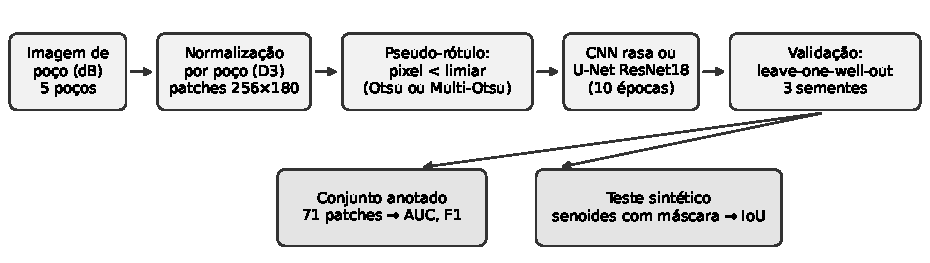
\includegraphics[width=\linewidth]{figuras/fig_metodo.pdf}
\caption{Visão geral do método. O pseudo-rótulo é gerado por limiar (Otsu; H11: Multi-Otsu), e a avaliação usa o conjunto anotado e o teste sintético.}
\label{fig:metodo}
\end{figure}

\subsection{Pseudo-rótulos e modelos}

O pseudo-rótulo de cada pixel é 1 se a amplitude normalizada fica abaixo do limiar de Otsu \cite{otsu1979} do poço. Foram usados dois modelos: uma CNN rasa com convoluções dilatadas (campo receptivo de $17 \times 17$) e uma U-Net \cite{ronneberger2015} com encoder ResNet18 \cite{he2016} pré-treinado, da biblioteca \textit{segmentation\_models\_pytorch} \cite{iakubovskii2019}. Como \textit{baselines}, usaram-se os limiares de Otsu, Multi-Otsu e K-means.

\subsection{Treino}

A perda é Dice mais entropia cruzada binária. O otimizador é Adam \cite{kingma2015}, com taxa de 1e-3, 1 época de aquecimento e decaimento cosseno, por 10 épocas, com parada antecipada pelo Dice contra o pseudo-rótulo do poço de validação. O aumento de dados é um deslocamento circular aleatório no azimute, e cada patch recebe 6 colunas circulares de cada lado (192 colunas). Cada configuração usa 3 sementes. Não houve ajuste de hiperparâmetros. \fonte{U13}

\subsection{Validação}

Foi usada a validação \textit{leave-one-well-out}: cada poço é o poço de teste uma vez, e o poço seguinte da lista é o de validação. Os patches que se sobrepõem aos anotados ficam fora do treino.

\subsection{Conjunto anotado}

Foram anotados 80 patches em duas rodadas (40 sorteados, 8 por poço, e 40 escolhidos entre os de pouca área escura). Cada patch recebe uma de três decisões: feição clara (55), sem feição (16) ou dúvida (9); restam 71 usáveis. Os critérios vêm de uma ficha baseada em Fioriti \cite{fioriti2026}. Uma reanotação às cegas de 10 patches, com mais de 10~h de intervalo e pela mesma pessoa, deu 10 de 10 respostas iguais (kappa de Cohen \cite{cohen1960} igual a 1,00; amostra pequena). O tatu22 não tem patch sem feição e o coala88 tem apenas 2. \fonte{itens 53 a 55; U8, U11}

\subsection{Métricas}

O escore de cada patch é a fração de pixels escuros (limiares) ou a probabilidade média prevista (modelos). Reportam-se a AUC e o F1 por patch contra a anotação, com IC de 95\% por \textit{bootstrap}. Os modelos e o Otsu são comparados nos mesmos patches por \textit{bootstrap} pareado da diferença de AUC.

\subsection{Teste sintético}

Senoides (1 ou 2 por patch, 1 volta completa, amplitude de 10 a 60 linhas, espessura de 4 a 8 linhas) são inseridas em fundos reais com pouca área escura. O contraste vale 0,25, 0,75 ou 0,95 vezes o limiar de Otsu do poço, com 24 fundos por contraste e por poço (72 patches por poço). Pixels já escuros no fundo ficam fora do cálculo. A máscara exata permite medir IoU e Dice por pixel. Os parâmetros são escolhas do autor, sem apoio de especialista, e cobrem só formas senoidais. \fonte{itens 64 a 66; U15}

\subsection{Ablações}

Cada ablação muda uma decisão e compara a U-Net com a referência, nas mesmas sementes e poços. Regra de leitura: há efeito se $|\text{média da diferença}|$ é maior que 1 desvio-padrão entre sementes e o sinal se repete em pelo menos 4 dos 5 poços; caso contrário, relata-se ``não foi detectada diferença''. A métrica principal é o IoU sintético. As ablações são: H4 (sem deslocamento circular), H5 (sem exclusão da D1), H3 (normalização global e por intervalo), H7 (encoder sem pré-treino), H11 (limiar Multi-Otsu no pseudo-rótulo, decisão do autor) e H9 (pseudo-rótulo gerado pelo Otsu binário da imagem reconstruída por um autoencoder convolucional de remoção de ruído \cite{silva2026}, treinado por poço, só na imagem do próprio poço, com 60 épocas; a entrada da U-Net continua a imagem normalizada). Como a H11 e a H9 mudam o pseudo-rótulo, o IoU sintético não vale para elas; a H11, a H9 e a H7 também são lidas pela AUC por \textit{patch} no conjunto anotado: há efeito se o intervalo de 95\% da diferença de AUC (\textit{bootstrap} pareado nos mesmos patches) exclui zero e a diferença média entre sementes passa de 1 desvio-padrão. \fonte{itens 79 e 80} As ablações H10, H8 e H6 do plano não foram executadas.

\subsection{Uso de ferramentas de IA}

Assistente de IA usado para apoio ao código e à revisão do texto. Decisões, experimentos e conclusões são do autor.

\section{Resultados}

\subsection{Baselines e modelos no conjunto anotado}

\begin{table}[ht]
\centering
\caption{AUC e F1 por patch no conjunto anotado (71 patches). Modelos: média $\pm$ desvio entre 3 sementes (AUC calculada por semente).}
\label{tab:anotado}
\begin{tabular}{lcc}
\toprule
Método & AUC & F1 \\
\midrule
Otsu & 0,932 (IC 0,856--0,988) & 0,920 \\
Multi-Otsu & 0,911 & 0,939 \\
K-means & 0,932 & 0,919 \\
CNN rasa & 0,800 $\pm$ 0,024 & 0,839 $\pm$ 0,052 \\
U-Net (ResNet18) & 0,806 $\pm$ 0,020 & 0,845 $\pm$ 0,041 \\
\bottomrule
\end{tabular}
\end{table}

A diferença pareada de AUC contra o Otsu, com o escore médio das 3 sementes em cada \textit{patch}, foi $-0{,}141$ (IC 95\%: $-0{,}242$ a $-0{,}062$) para a CNN rasa (AUC 0,791) e $-0{,}123$ ($-0{,}213$ a $-0{,}050$) para a U-Net (AUC 0,809). Nesta configuração, os dois modelos ficaram abaixo do Otsu. A diferença entre a U-Net e a CNN rasa é pequena, e o teste tem pouco poder para detectá-la. A AUC mede a concordância com as anotações, e o sinal ``escuro'' é o mesmo no limiar e na anotação. \fonte{itens 60 a 63; U9, U14}

\subsection{Teste sintético}

\begin{table}[ht]
\centering
\caption{IoU no teste sintético, por contraste (referência; 3 sementes, 5 poços).}
\label{tab:sint}
\begin{tabular}{lccc}
\toprule
Contraste & CNN rasa & U-Net & Otsu \\
\midrule
0,25 $\times$ limiar & 0,911 & 0,909 & 1,000 \\
0,75 $\times$ limiar & 0,905 & 0,887 & 1,000 \\
0,95 $\times$ limiar & 0,503 & 0,518 & 0,946 \\
Total & 0,773 $\pm$ 0,021 & 0,771 $\pm$ 0,021 & 0,982 \\
\bottomrule
\end{tabular}
\end{table}

O Otsu é a regra que gerou o pseudo-rótulo, e o teste sintético a favorece por construção em contrastes bem abaixo do limiar. O Dice dos modelos contra o pseudo-rótulo foi 0,680 $\pm$ 0,025 (CNN rasa) e 0,625 $\pm$ 0,011 (U-Net), com variação grande entre poços (de cerca de 0,41 a 0,86), cuja causa não foi investigada. \fonte{item 67}

\subsection{Ablações}

\begin{table}[ht]
\centering
\caption{Ablações da U-Net contra a referência (IoU sintético, média de 3 sementes e 5 poços; referência: 0,771). Dif.: candidata menos referência; DP: desvio entre sementes.}
\label{tab:abl}
\small
\begin{tabular}{lcccl}
\toprule
Ablação & Dif. & DP & Poços & Leitura \\
\midrule
H4 sem deslocamento & $-0{,}008$ & 0,043 & 3/5 & sem diferença detectada \\
H5 sem exclusão D1 & $-0{,}008$ & 0,042 & 3/5 & sem diferença detectada \\
H3 global\textsuperscript{a} & $-0{,}251$ & 0,057 & 4/5 & inconclusiva \\
H3 por intervalo\textsuperscript{a} & $-0{,}406$ & 0,020 & 5/5 & inconclusiva \\
H7 sem pré-treino & $-0{,}013$ & 0,030 & 2/5 & sem diferença detectada \\
\bottomrule
\end{tabular}
\\[2pt]
\footnotesize \textsuperscript{a}Teste sintético comum, gerado uma vez com o limiar da referência. \fonte{itens 75 e 77; código em \texttt{src/synth/comum.py}; conferência na seção 5.10 do notebook 05}
\end{table}

Observou-se que a remoção do deslocamento circular (H4) e a remoção da exclusão das zonas de artefato (H5) mudaram o IoU sintético em $-0{,}008$, abaixo do desvio entre sementes; na H7, a mudança foi de $-0{,}013$ (0,771 para 0,758; desvio de 0,030). Não foi detectada diferença nas três ablações. Nas duas normalizações alternativas (H3), o IoU sintético ficou abaixo da referência no teste comum; em um teste anterior, com o limiar de cada configuração, a normalização por intervalo tinha ficado acima ($+0{,}129$). O sinal mudou com o teste, e por isso a H3 fica inconclusiva. O teste comum usa o limiar da referência para definir as feições, o que sugere um viés a favor dela; na H3 por intervalo, o IoU ficou quase igual nos três contrastes (0,368, 0,369 e 0,360), o que sugere que a saída responde pouco à feição inserida. As duas hipóteses não foram testadas. \fonte{H4, H5 e o teste com limiar próprio: item 74; teste comum: item 77; H7: item 82}

\begin{table}[ht]
\centering
\caption{AUC por \textit{patch} no conjunto anotado (71 \textit{patches}; escore médio das 3 sementes; Otsu: 0,932). Diferenças com IC de 95\% por \textit{bootstrap} pareado nos mesmos patches.}
\label{tab:auc}
\footnotesize
\begin{tabular}{lccc}
\toprule
Configuração & AUC & Dif. para a referência & Dif. para o Otsu \\
\midrule
Referência & 0,809 & --- & $-0{,}123$ ($-0{,}213$ a $-0{,}050$) \\
H7 sem pré-treino & 0,810 & $+0{,}001$ ($-0{,}072$ a $0{,}073$) & $-0{,}122$ ($-0{,}203$ a $-0{,}046$) \\
H11 Multi-Otsu & 0,923 & $+0{,}114$ (0,046 a 0,200) & $-0{,}009$ ($-0{,}052$ a 0,031) \\
H9 autoencoder & 0,849 & $+0{,}040$ ($-0{,}007$ a 0,097) & $-0{,}083$ ($-0{,}170$ a $-0{,}016$) \\
\bottomrule
\end{tabular}
\end{table}

\begin{figure}[t]
\centering
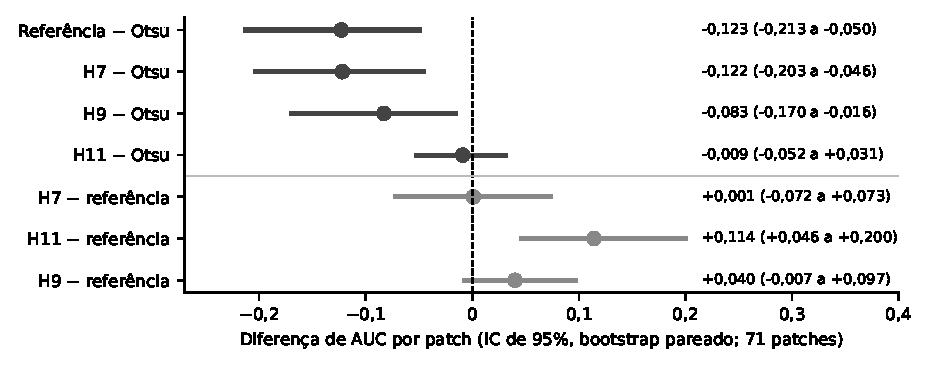
\includegraphics[width=\linewidth]{figuras/fig_auc.pdf}
\caption{Diferenças de AUC por \textit{patch} com IC de 95\% (\textit{bootstrap} pareado nos mesmos 71 \textit{patches}). Linhas superiores: contra o Otsu; inferiores: contra a referência.}
\label{fig:auc}
\end{figure}

A H11 troca o limiar do pseudo-rótulo: em vez do Otsu binário, usa o limiar que separa a classe mais escura do Multi-Otsu com três classes, o que marca de 3\% a 6\% dos pixels como escuros, contra 3,5\% a 52,1\% na referência. Observou-se AUC de 0,923 contra 0,809 da referência, com diferença pareada de $+0{,}114$ (IC de 95\% de 0,046 a 0,200), acima do desvio entre sementes (0,020); a regra de leitura indica efeito. A AUC mede a concordância com o critério ``zona escura clara'', próximo do que o pseudo-rótulo marca, e não mostra melhor segmentação geológica. Contra o Otsu nos mesmos patches (Tabela~\ref{tab:auc}), a referência e a H7 ficaram abaixo ($-0{,}123$ e $-0{,}122$, com intervalos que excluem zero); para a H11, não foi detectada diferença ($-0{,}009$; IC de 95\% de $-0{,}052$ a 0,031). Com 71 \textit{patches}, o intervalo é largo, e isso não prova equivalência.

Na H9, as frações de pixels escuros do pseudo-rótulo ficaram perto das da referência (diferença de $+0{,}001$ a $+0{,}023$). A AUC foi de 0,849, com diferença pareada de $+0{,}040$ (IC de 95\% de $-0{,}007$ a 0,097); a diferença média entre sementes ($+0{,}037$) passa de 1 desvio (0,027), mas o intervalo inclui zero, e por isso não foi detectada diferença. A estimativa é positiva nas três sementes; com 71 \textit{patches}, o poder é baixo, e um efeito pequeno não é excluído. Contra o Otsu, a H9 ficou abaixo ($-0{,}083$). \fonte{itens 87 a 89} \fonte{item 82 e seção 5.16 do notebook 05; fração escura: item 76}

\section{Discussão}

Com o pseudo-rótulo do Otsu binário, a CNN rasa e a U-Net ficaram abaixo do Otsu na AUC por \textit{patch} (Tabelas~\ref{tab:anotado} e~\ref{tab:auc}). Este trabalho não testa a causa. Três hipóteses ficam abertas: o pseudo-rótulo é ruidoso, 10 épocas são poucas, e os hiperparâmetros não foram ajustados. A ablação H11 dá um indício sobre a primeira: com o limiar Multi-Otsu no pseudo-rótulo, não foi detectada diferença para o Otsu. Isso sugere que a definição de ``escuro'' do pseudo-rótulo limita os modelos da referência. Um sinal compatível: no tatu22, o limiar de Otsu separa regimes de amplitude (Seção~\ref{sec:lim}). \fonte{U12, U23; item 76}

Nas ablações do deslocamento circular (H4), da exclusão das zonas de artefato (H5) e do pré-treino (H7), não foi detectada diferença. Com 3 sementes e 5 poços, o poder é baixo, e isso não prova ausência de efeito. A normalização (H3) ficou inconclusiva, porque o teste sintético depende do limiar que define ``escuro''.

A comparação com trabalhos anteriores é só qualitativa. Silva \cite{silva2026} mede a concordância com o próprio pseudo-rótulo e relata, na média entre poços, 0,614 para o Otsu na imagem bruta e 0,703 após o autoencoder; este trabalho mede a AUC contra uma anotação independente. Métricas, classes e dados diferem, e os valores não se comparam. Anjos et al. \cite{anjos2022} usam dados privados e outra tarefa (\textit{breakouts}), e o IoU deles varia de 33,3\% a 70,0\% entre dobras separadas por poço. A H9 mostra que a limpeza da imagem por autoencoder, sem mudar a definição de ``escuro'', não teve diferença detectada para a referência e continuou abaixo do Otsu. Esse contraste com a H11 sugere que o limiar pesa mais que a limpeza do rótulo, sem teste com outros limiares.

\section{Limitações}\label{sec:lim}

\begin{itemize}
\item \textbf{Escopo e anotações.} A segmentação é binária e não distingue fraturas, cavidades, \textit{breakouts} e artefatos. As 80 anotações vêm de uma só pessoa, sem especialista, com critérios de uma fonte principal \cite{fioriti2026}; a fonte original sobre artefatos \cite{lofts1999} não foi consultada. A reanotação (10 \textit{patches}) é um indicador grosso. \fonte{U7, U8, U18}
\item \textbf{Circularidade e amostra.} O critério de anotação (``zona escura clara'') e o escore do limiar usam o mesmo sinal; a AUC mede a concordância com esse critério, e não a qualidade geológica. Os 9 \textit{patches} em dúvida ficaram fora, o que pode tornar o teste mais fácil. São 71 \textit{patches}, e o tatu22 não tem exemplos negativos; o poder estatístico é baixo. \fonte{U9, U11, U14}
\item \textbf{Pseudo-rótulo e treino.} O pseudo-rótulo inclui sombras e artefatos. O limiar de Otsu separa regimes de amplitude: 56,5\% dos \textit{patches} válidos do tatu22 têm mais de 50\% de pixels marcados (8,9\% no coala88 e 4,2\% no botorosa47), e a causa física não foi investigada. Foram usadas 10 épocas e hiperparâmetros fixos. Só um limiar alternativo (H11) foi testado, sem fonte de especialista, e o autoencoder (H9) foi treinado por poço, e não por intervalo como em Silva \cite{silva2026}. \fonte{U12, U13, U23}
\item \textbf{Teste sintético e normalização (H3).} Parâmetros escolhidos pelo autor; só formas senoidais. O IoU sintético usa o limiar da referência para definir as feições: com um teste diferente por configuração, a normalização por intervalo ficou acima da referência, e com um teste comum, abaixo. O resultado depende do teste e não ordena as normalizações; uma medida sem limiar (AUC por pixel) não foi feita. \fonte{U15, U22, U24}
\item \textbf{Generalização.} Cinco poços de uma mesma empresa e região. \fonte{U19}
\end{itemize}

\section{Conclusão}

Com base nos resultados deste trabalho, em 71 \textit{patches} anotados e 5 poços:
\begin{enumerate}
\item Com o pseudo-rótulo do Otsu binário, a CNN rasa e a U-Net ficaram abaixo do Otsu na AUC por \textit{patch}, com diferenças pareadas de $-0{,}141$ e $-0{,}123$ (Tabela~\ref{tab:anotado}).
    \item Com o limiar Multi-Otsu no pseudo-rótulo, não foi detectada diferença para o Otsu ($-0{,}009$; IC de 95\% de $-0{,}052$ a 0,031), e o ganho sobre a referência foi de $+0{,}114$ (Tabela~\ref{tab:auc}). Isso sugere que a definição de ``escuro'' do pseudo-rótulo pesa mais que as outras decisões testadas.
\item Não foi detectada diferença nas ablações do deslocamento circular (H4), da exclusão das zonas de artefato (H5), do pré-treino (H7) e do pseudo-rótulo por autoencoder (H9); a normalização (H3) ficou inconclusiva (Tabelas~\ref{tab:abl} e~\ref{tab:auc}).
\end{enumerate}
Os resultados valem para esta configuração (10 épocas, hiperparâmetros fixos, anotação de uma pessoa, sem especialista) e para o WAID.

\section*{Disponibilidade}

Código sob a licença Apache 2.0; repositório: \url{https://github.com/jorgesouza63/puc_pel_mel_sit_ele2346}. Sementes e tabelas ficam no repositório. Dados: WAID/PETROBRAS, CC BY 4.0 \cite{waid}.

\bibliographystyle{sbc}
\bibliography{referencias}

\end{document}
